\documentclass[10pt]{bmc_article}

% Load packages
\usepackage{cite} % Make references as [1-4], not [1,2,3,4]
\usepackage{url}  % Formatting web addresses
\usepackage{ifthen}  % Conditional
\usepackage{multicol}   %Columns
\usepackage[utf8]{inputenc} %unicode support
\urlstyle{rm}

%%%%%%%%%%%%%%%%%%%%%%%%%%%%%%%%%%%%%%%%%%%%%%%%%
%%                                             %%
%%  If you wish to display your graphics for   %%
%%  your own use using includegraphic or       %%
%%  includegraphics, then comment out the      %%
%%  following two lines of code.               %%
%%  NB: These line *must* be included when     %%
%%  submitting to BMC.                         %%
%%  All figure files must be submitted as      %%
%%  separate graphics through the BMC          %%
%%  submission process, not included in the    %%
%%  submitted article.                         %%
%%                                             %%
%%%%%%%%%%%%%%%%%%%%%%%%%%%%%%%%%%%%%%%%%%%%%%%%%
\usepackage{graphicx}
%\def\includegraphic{}
%\def\includegraphics{}

\setlength{\topmargin}{0.0cm}
\setlength{\textheight}{21.5cm}
\setlength{\oddsidemargin}{0cm}
\setlength{\textwidth}{16.5cm}
\setlength{\columnsep}{0.6cm}

\newboolean{publ}

%%%%%%%%%%%%%%%%%%%%%%%%%%%%%%%%%%%%%%%%%%%%%%%%%%
%%                                              %%
%% You may change the following style settings  %%
%% Should you wish to format your article       %%
%% in a publication style for printing out and  %%
%% sharing with colleagues, but ensure that     %%
%% before submitting to BMC that the style is   %%
%% returned to the Review style setting.        %%
%%                                              %%
%%%%%%%%%%%%%%%%%%%%%%%%%%%%%%%%%%%%%%%%%%%%%%%%%%

%Review style settings
\newenvironment{bmcformat}{\begin{raggedright}
\baselineskip20pt\sloppy\setboolean{publ}{false}}{\end{raggedright}
\baselineskip20pt\sloppy}

%Publication style settings
%\newenvironment{bmcformat}{\fussy\setboolean{publ}{true}}{\fussy}

%New style setting
%\newenvironment{bmcformat}{\baselineskip20pt\sloppy\setboolean{publ}{false}}{
%\baselineskip20pt\sloppy}

% Begin ...
\begin{document}
\begin{bmcformat}


%%%%%%%%%%%%%%%%%%%%%%%%%%%%%%%%%%%%%%%%%%%%%%
%%                                          %%
%% Enter the title of your article here     %%
%%                                          %%
%%%%%%%%%%%%%%%%%%%%%%%%%%%%%%%%%%%%%%%%%%%%%%

\title{Avogadro: An Advanced Semantic Chemical Editor, Visualization, and
  Analysis Platform}

%%%%%%%%%%%%%%%%%%%%%%%%%%%%%%%%%%%%%%%%%%%%%%
%%                                          %%
%% Enter the authors here                   %%
%%                                          %%
%% Ensure \and is entered between all but   %%
%% the last two authors. This will be       %%
%% replaced by a comma in the final article %%
%%                                          %%
%% Ensure there are no trailing spaces at   %%
%% the ends of the lines                    %%
%%                                          %%
%%%%%%%%%%%%%%%%%%%%%%%%%%%%%%%%%%%%%%%%%%%%%%
\author{Marcus D Hanwell\correspondingauthor$^{1, 2}$%
  \email{Marcus D Hanwell\correspondingauthor - marcus.hanwell@kitware.com}
  \and
  Donald E Curtis$^3$%
  \and
  David Lonie$^4$%
  \and
  Tim Vandermeersch$^5$%
  \and
  Eva Zurek$^4$%
  \and
  Geoffrey R Hutchison$^1$%
  \email{Geoffrey R Hutchison - geoffh@pitt.edu}
  }

%%%%%%%%%%%%%%%%%%%%%%%%%%%%%%%%%%%%%%%%%%%%%%
%%                                          %%
%% Enter the authors' addresses here        %%
%%                                          %%
%%%%%%%%%%%%%%%%%%%%%%%%%%%%%%%%%%%%%%%%%%%%%%

\address{%
  \iid(1)Department of Chemistry, University of Pittsburgh, 219 Parkman Avenue,
Pittsburgh, PA, 15260, USA\\
  \iid(2)Department of Scientific Computing, Kitware, Inc., 28 Corporate Drive,
Clifton Park, NY, 12065, USA\\
  \iid(3)Department of Computer Science, Coe College, 1220 First Avenue NE,
Cedar Rapids, Iowa 52402\\
  \iid(4)Department of Chemistry, State University of New York at Buffalo,
Buffalo, New York 14260-3000\\
  \iid(5)Avogadro development team
}%

\maketitle

%%%%%%%%%%%%%%%%%%%%%%%%%%%%%%%%%%%%%%%%%%%%%%
%%                                          %%
%% The Abstract begins here                 %%
%%                                          %%
%% Please refer to the Instructions for     %%
%% authors on http://www.biomedcentral.com  %%
%% and include the section headings         %%
%% accordingly for your article type.       %%
%%                                          %%
%%%%%%%%%%%%%%%%%%%%%%%%%%%%%%%%%%%%%%%%%%%%%%

\begin{abstract}

\textbf{Background:} The Avogadro project is an advanced molecule editor and
visualizer
designed for cross-platform use in computational chemistry, molecular
modeling, bioinformatics, materials science, and related areas. It
offers flexible high quality rendering and a powerful plugin
architecture. Typical uses include building molecular structures,
formatting input files, and analyzing output of a wide variety of
computational chemistry packages. By using the CML file format as its native
document type, Avogadro seeks to enhance the semantic accessibility of
chemical data types.

\textbf{Results:} The work presented here details the Avogadro library, which
provides a framework,
application programming interface, and three-dimensional visualization
capabilities, and has direct applications to research and education in the
fields of chemistry, physics, materials science, and biology. The Avogadro
application provides a rich graphical interface using dynamically loaded
plugins through the library itself. The application and library can
each be extended by implementing a plugin module in C++
or Python to explore different visualization techniques,
build/manipulate molecular structures, and interact with other programs.
We describe some example extensions, one which uses a genetic algorithm to find
stable crystal structures, and one which interfaces with the PackMol program to
create packed, solvated structures for molecular dynamics simulations.

\textbf{Conclusions:} It is freely available under an open-source license from
http://avogadro.openmolecules.net.

\end{abstract}

\ifthenelse{\boolean{publ}}{\begin{multicols}{2}}{}

\section{Introduction}

Many areas such as chemistry, materials science, physics, and biology need
efficient computer programs to both build and visualize molecular structures.
The field of molecular graphics is dominated by viewers with little or no
editing capabilities, such as RasMol~\cite{RasMol}, JMol~\cite{JMol},
PyMOL~\cite{PyMOL}, VMD~\cite{VMD}, QuteMol~\cite{QuteMol}, and
BALLView~\cite{BALLView} among many others. The aforementioned viewers are all
freely available, and most of them are available under open source licenses and
work on the most common operating systems (GNU/Linux, Apple Mac OS X, Windows,
and BSD).

The choice of software capable of building chemical structures is far smaller.
There are existing commercial packages, such as Spartan, CAChe, GaussView,
Materials Studio~\cite{Accelrys} and CrystalMaker~\cite{CrystalMaker}, that are
polished and capable of constructing many different types of molecular
structures. They are, however, not available for all operating systems (most of
them only run on Microsoft Windows), and are not easily extensible, customized,
or integrated into automated workflows. Licensing costs can be prohibitive. If
the company were to change its direction or focus this can lead to a loss of
significant research investment in a commercial product.

The selection of free, open source, cross platform molecular builders was quite
limited when the Avogadro project was founded in late 2006.
Ghemical~\cite{Ghemical} was one of the only projects satisfying these needs at
the time. Two of the authors (Hutchison and Curtis) contributed to Ghemical
previously, but had found that it was not easily extensible. This led them to
found a new project to address the issues they had observed in Ghemical
and other packages. The Molden~\cite{Molden} application was also available,
able to build up small molecules and analyze output from several quantum codes.
It suffers from a restrictive license and it uses an antiquated graphical
toolkit, which is not native on most modern operating systems.

Broad goals for the design of a molecular editor were identified following a
case study of the available applications. One of the main issues with both
commercial and open source applications is a lack of extensibility, many of the
applications also only work on one or two operating systems. An open and
extensible framework is needed to perform innovative research. The
creation of such a framework that implements many of the necessary foundations
for a molecular builder and visualizer would facilitate more effective research
in this area.

At the time of writing it is apparent that other researchers have perceived
similar needs. Several new applications are available today that focus on both
building and visualizing molecular structure. These include
CCP1GUI~\cite{CCP1GUI}, Gabedit~\cite{Gabedit} along with some highly specific
editors such as MacMolPlt~\cite{MacMolPlt} which focus on particular
computational packages (i.e., GAMESS-US for MacMolPlt). Whilst offering many
interesting and
useful features, these projects suffer from the same issues centering
around effective reuse of existing code, well commented and documented code, and
easy extension to add new features and adapt for specialized areas.

The Avogadro project was started in earnest in 2007, and over the
first 5 years of development has been downloaded over 250,000
times~\cite{Downloads}, been translated into over 20
languages~\cite{Translations}, and has over 20
contributors~\cite{OhlohContributors}. From the beginning, the project
has strived to make a robust, flexible framework for
both building and visualizing molecular structures. Much of the initial focus
has been placed on preparing input and analyzing output from quantum
calculations. Other applications such as preparing input for MD simulations and
visualizing periodic structures will also be presented, demonstrating the
flexibility of the Avogadro platform. The software has been developed by
members of the Blue Obelisk movement, following the three pillars outlined by
the group: Open Data, Open Standards and Open Source~\cite{BlueObelisk2006,
BlueObelisk2011}.

\section{The Graphical User Interface}

The first thing most people will see is the main Avogadro application
window, as shown in Figure~\ref{f:avogadrogui}.
Binary installers are provided under the GPL license for Apple Mac OS X and
Microsoft Windows, along with packages for all of the major Linux distributions.
This means that Avogadro can be installed quite easily on most operating
systems. Easy to follow instructions on how to compile the latest source code
are also provided on the main Avogadro web
site\cite{CompileWindows}\cite{CompileLinux} for the more adventurous,
or those using an operating system that is not yet supported.

\begin{figure}
  \begin{center}
    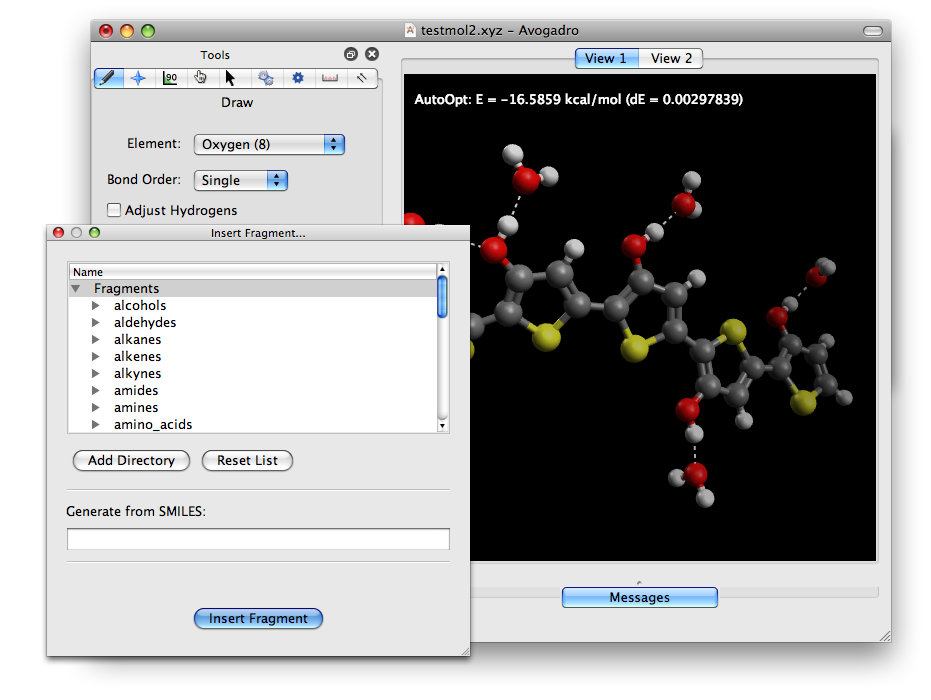
\includegraphics[width=0.9\textwidth]{images/avogadro-drawing}
  \end{center}
  \caption{The Avogadro graphical user interface (on Mac OS X), showing the
editing interface
for a molecule.}
  \label{f:avogadrogui}
\end{figure}

The Qt toolkit from Nokia gives Avogadro a native look and feel on the three
supported operating systems---Linux, Mac OS X and Windows. The basic
functionality expected in a molecular builder and viewer has been implemented,
along with several less common features. It is very easy for new users to
install Avogadro and build their
first molecules within minutes. Thanks to the Open Babel library Avogadro
supports a large portion of the chemical file formats that are in
common use.

The vast majority of this functionality has been written using the
interface made available to plugin writers, and is loaded at
runtime. We will discuss these plugin interfaces and descriptions of
the plugin types later.

\section{Semantic Chemistry}

Avogadro has used CML~\cite{CML2011a, CML2011b} as its default file format from
a very early stage, this
was chosen over all the other file formats provided by Open Babel due to the
semantic structure provided and the support available in Open Babel. The CML
format offers a number of advantages over others in common use, including the
ability to extend the format to include more information and add the features
necessary in an application at a later time by looking for new parts of the
standard.

Through the use of Open Babel a large array of file formats can be interpreted,
and a large amount of the work in doing this has been done by the Open Babel
project. When extending Avogadro to read in larger amounts of the output from
quantum codes, it was necessary to devote significant development resources to
understanding and adding meaning to the quantum code outputs. This work was
developed in a plugin, which was later split out into a small independent
library called OpenQube. More recently a great deal of work has been done
by the Quixote project~\cite{Quixote}, JUMBO-Converters and the Semantic
Physical Science workshop to augment qunatum codes to output more of this data
directly from the code. If CML can be extended, it is possible to reuse
existing conventions for molecular structure data, and add new conventions for
the additional quantum data.

\subsection{Building a Molecule: Atom by Atom}

After opening Avogadro a window such as that shown in Figure~\ref{f:avogadrogui}
is presented. By default, the draw tool is selected. Simply left clicking on the
black part of the display
allows the user to draw a carbon atom. If the user pushes the left
mouse button down and drags a bonded carbon atom would be drawn
between the start point and the final position where the mouse was released.

A large amount of effort has been expended to create an intuitive tool for
drawing small molecules. Common elements can be selected from a drop down list,
or a periodic table can be displayed to select less common elements. Clicking on
an existing atom changes its type, dragging reverts the original atom and draws
the new atom bonded to the original. If the bonds are left-clicked then the bond
order cycles between single, double and triple. Similarly, typing the
atomic symbol (e.g., ``C-o'' for cobalt) changes the selected element,
or typing the numbers ``1'', ``2'', and ``3'' changes the bond order.

Right clicking on atoms or bonds deletes them. If the ``Adjust Hydrogens'' box
is checked, the number of hydrogens bonded to each atom is automatically
adjusted to satisfy valency. Alternatively, this can also be done at the end of
an editing session by using the add hydrogens extension in the build menu.

In addition to the draw tool there are two tools for adjusting the position of
atoms in existing molecules. The ``atom centric manipulate'' tool can be used to
move an atom or a group of selected atoms. The ``bond centric manipulate'' tool
can
be used to select a bond and then adjust all atoms positions relative to the
selected bond in various ways (e.g., altering the bond length, bond
angles, or dihedral angles). These three tools allow for a great deal of
flexibility in building small molecules interactively on screen.

Once the molecular structure is complete the forcefield extension can be used to
perform a geometry optimization. By clicking on ``Extensions'' and ``Optimize
Geometry'' a fast geometry optimization is performed on the molecule. The
forcefield and calculation parameters can be adjusted, but the defaults are
adequate for most molecules. This workflow is typical when building up a small
molecular structures for use as input to quantum calculations, or publication
quality figures.

An alternative is to combine the ``Auto Optimization'' tool with the drawing
tool. This presents a unique way of sculpting the molecule while the geometry is
constantly minimized in the background. The geometry optimization is animated,
and the effect of changing bond orders, adding new groups or removing groups can
be observed interactively.

Several dialogs are implemented to provide information on molecule properties,
and
to precisely change parameters, such as the cartesian coordinates of the atoms
in the molecule.

\subsection{Building a Molecule: From Fragments} %Geoff?

\begin{figure}
  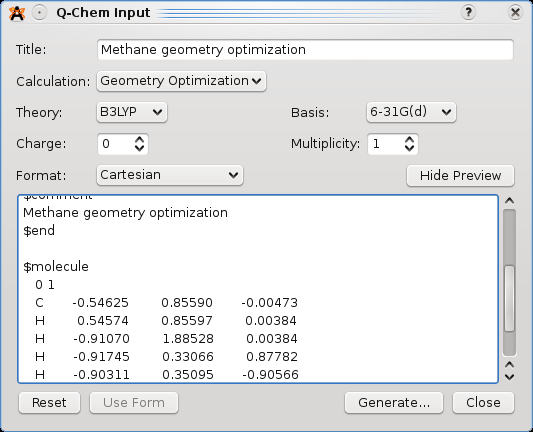
\includegraphics[width=0.44\textwidth]{images/avogadro-q-chem}
  \hspace{0.1cm}
  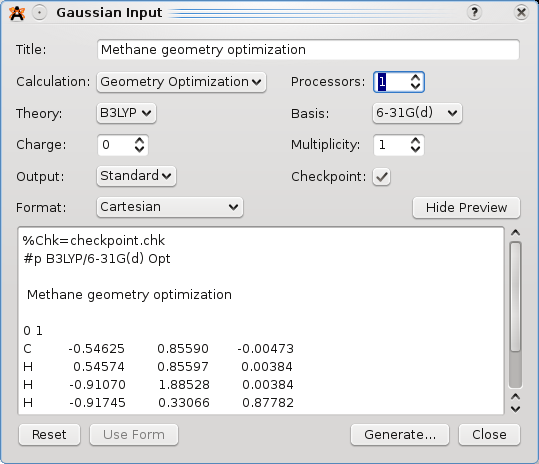
\includegraphics[width=0.44\textwidth]{images/avogadro-gaussian}
  \caption{Dialog for generating input for Q-Chem (left) and Gaussian (right).
    Note that both dialogs are similar in interface, allowing users to use
    multiple computational chemistry packages.}
  \label{f:quantumdialogs}
\end{figure}

\subsection{Preparing Input for Quantum Codes}

Several extensions were developed for Avogadro that assist the user in preparing
input files for popular quantum codes such as GAMESS-US, Gaussian, Q-Chem, and
MOPAC. The graphical dialogs present the features required to run basic quantum
calculations, some examples are shown in figure~\ref{f:quantumdialogs}.

The preview of the input file at the bottom of each dialog is updated as options
are changed. This approach helps new users of quantum codes to learn the syntax
of input files for different codes, and to quickly generate useful input files
as they learn. The input can be edited in the dialog before the file is saved
and submitted to the quantum code. The MOPAC extension can also run the  MOPAC
program directly, if it is available on the user's computer, and then reload the
output file into Avogadro once the calculation is complete.

\subsection{Alignment and Measurements}

One of the specialized tools included in the standard Avogadro distribution is
the alignment tool. This mouse tool facilitates the alignment of a molecular
structure with the coordinate origin if one atom is selected, and along the
specified axis if two atoms are selected. The alignment tool can be combined
with the measure, select and manipulate tools to create inputs for
quantum codes where the position and orientation of the molecule is important.
One example of this is calculations where an external electric field is applied
to the molecule. In these types of calculations the alignment of the molecule
can have a large effect.

More complex alignment tools for specific tasks could be created. The alignment
tool was created in just a few hours for a specific research project performing
calculation on the piezoelectric effect in single molecules. This is a prime
example where extensibility was very important to perform
research using a graphical computational chemistry tool. It would not have been
worth the investment to create a new application just to align molecular
structures to an axis, but creating a plugin for an extensible project was not
unreasonable.


\section{Visualization}

The Avogadro application uses OpenGL to render molecular representations to the
screen interactively. OpenGL offers a good cross platform API for rendering
three dimensional images using hardware accelerated graphics. OpenGL
1.1 and below is used in most of the rendering code, and so Avogadro can be used
even on very modest/old computer systems. It is capable of taking advantage of
some of the newer features available in OpenGL 2.0, but this has been kept as an
optional extra feature when working on novel visualizations of molecular
structure.

\subsection{Standard Representations}

\begin{figure}
  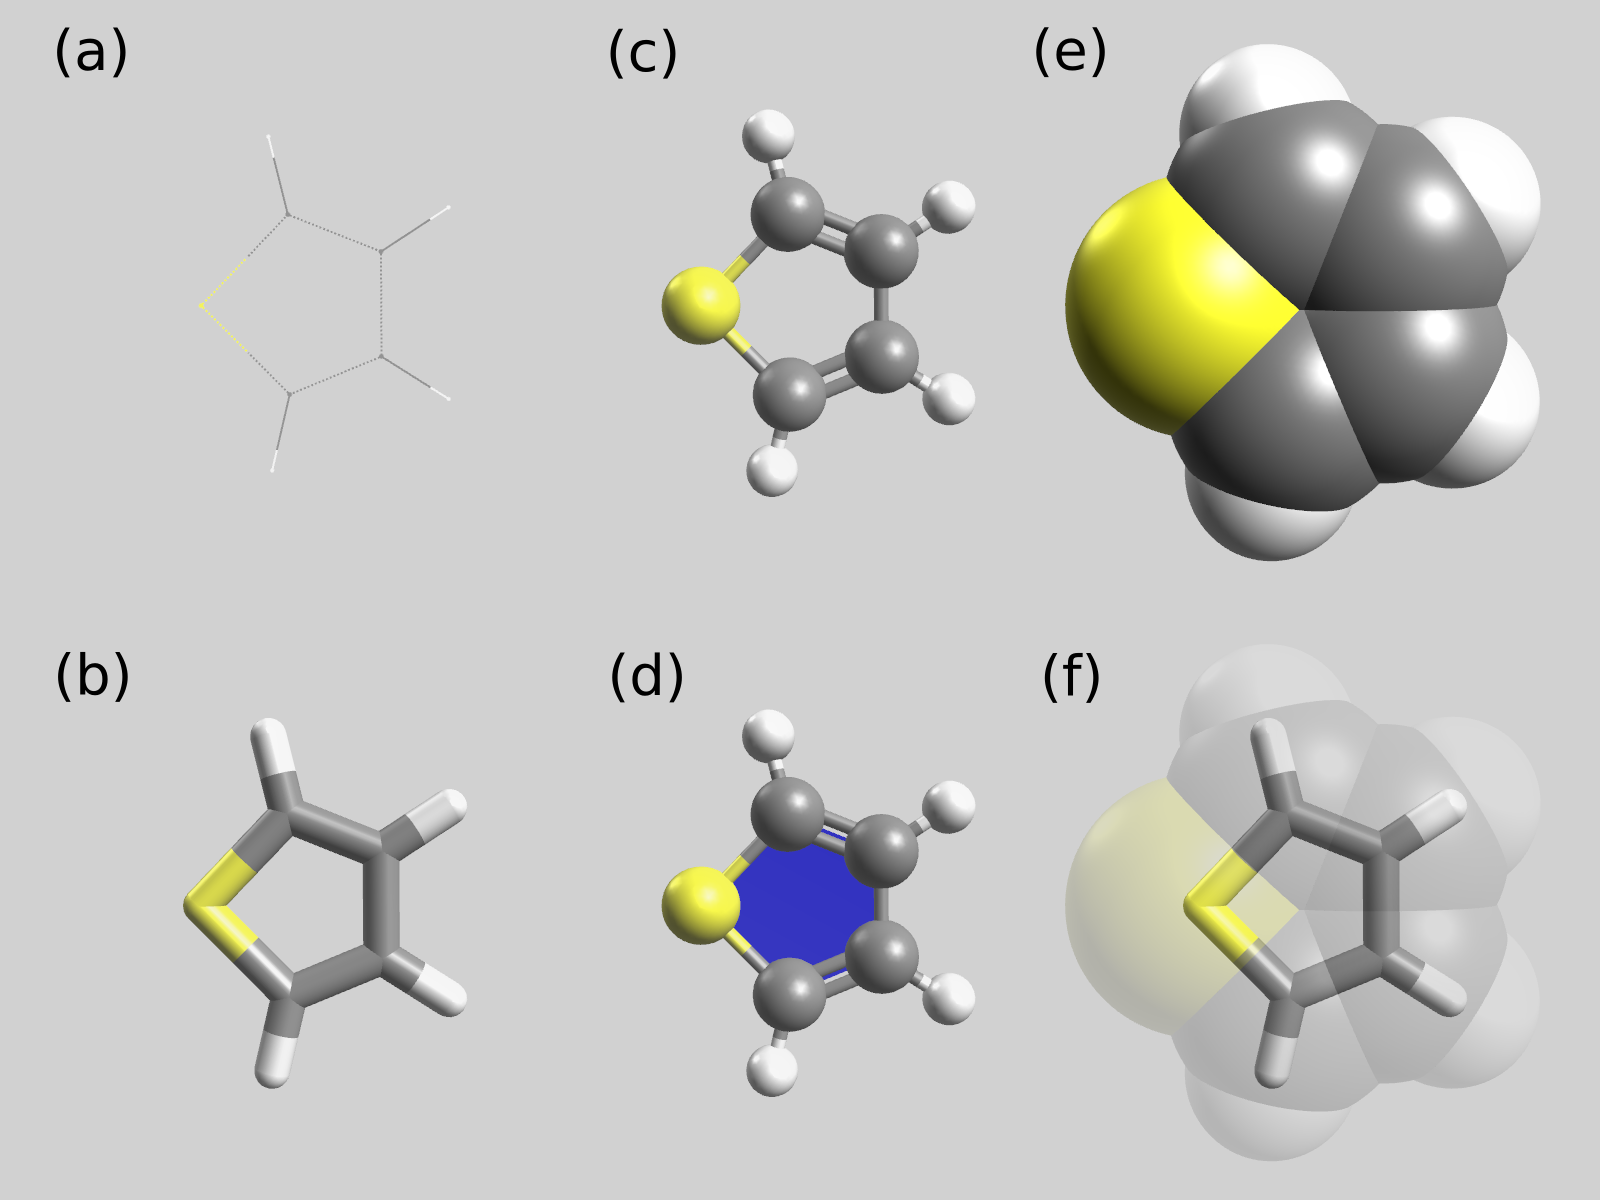
\includegraphics[width=0.95\textwidth]{images/standardRepsLabel}
  \caption{Several molecular representations of thiophene, (a) wireframe,
    (b) stick/liquorice, (c) ball and stick, (d) ball and stick with ring,
    (e) Van der Waals/CPK and (f) transparent Van der Waals with stick.}
  \label{f:standardReps}
\end{figure}

In chemistry there are several standard representations of molecular structure,
originally based upon those possible with physical models. The Avogadro
application implements each of these representations shown in
figure~\ref{f:standardReps} as a plugin. These range from the simple wireframe
representation, stick/licorice, ball and stick and Van der Waals spheres.

It is also possible to combine several representations, such as ball and stick
with ring rendering, figure~\ref{f:standardReps} (d), and a semi-transparent Van
der Waals space-filling representation with a stick representation to elucidate
molecular backbone, figure~\ref{f:standardReps} (f).

\subsection{Electronic Structure}

The support for electronic structure visualization evolved in Avogadro.
Initially support for reading in Gaussian cube files was added to Open Babel,
and a marching cubes implementation was added to Avogadro to visualize
isosurfaces. Once this was integrated it became clear that many codes could not
easily produce cube files, and that direct support for calculating cubes in the
Avogadro application would be advantageous.

Initially support for Gaussian type orbitals was added, as used in a large
range of quantum codes. Later support for Slater type orbitals was added in
order to visualize the output from the MOPAC code. This code was written using
the Qt Concurrent framework, reading in the basis set, eigenvectors, and density
matrix to directly calculate molecular orbitals and electron
densities. The cube calculation is highly multithreaded, parallelizing the
calculation of each point in the regular grid making up the volume of interest.
The original marching cubes implementation is then used to calculate
isosurfaces in much the same way as for Gaussian cube files.

Both features were developed within plugins, and matured there. More recently
the code responsible for reading quantum output files and calculating the cubes
has been separated out into a separate library called ``OpenQube''. This allows
other applications to reuse the code more easily, as well as facilitating its
use on clusters where graphical rendering may not be available. A range of
output files are supported including Gaussian formatted checkpoint files,
Q-Chem formatted checkpoints, GAMESS, Molpro and MOPAC AUX files. There are
several related projects to add semantic meaning to this type of output,
including the JUMBO-Converters project and Quixote.

\subsection{Secondary Biological Structure}

Avogadro uses the PDB reader from Open Babel, and is able to to visualize the
secondary structure annotated in those files. Initially a simple plugin was
developed that drew a simple tube between the biomolecule backbone, then a
second more advanced visualization plugin was developed to calculate meshes for
the alpha helices and beta sheets. The simple plugin is much faster, but with
more optimization it is clear that the superior rendering produces the results
expected in that field.

\subsection{GLSL, Novel Visualization}

GLSL, or OpenGL Shader Language, is a C-like syntax that can be used to develop
code that will run on graphics cards. It has been used to great effect by the
games industry, as well as in many areas of data visualization. Several recent
papers highlight the potential in chemistry, such as QuteMol~\cite{QuteMol} in
adding support for features such as ambient occlusion to add depth to images.

Avogadro has support for vertex and fragment shader programs, and several
examples are bundled with Avogadro. If the user's graphics card is capable,
these programs can be loaded at runtime and used to great effect to visualize
structure. Some of these include summarization techniques such as isosurface
rendering where only the edges orthogonal to the view plane are visible giving
a much better rendering of both the molecular and electronic structure.

\subsection{Ray Tracing}

Avogadro uses a painter abstraction that makes it much easier for developers to
add new display types. It also abstracts away the renderer, making it possible
to add support for alternative backends. Currently only OpenGL and POV-Ray are
supported. Due to the abstraction we are able to use the implicit surfaces
available in ray tracers to render molecular structure at very high levels of
clarity with none of the triangle artifacts present in standard OpenGL rendered
images. Much higher quality transparency and reflection also allow for the
images to be used in poster and oral presentations as well as research
articles.

This feature is implemented in an extension, with an additional painter class
deriving from the base class and a dialog allowing the user to edit the basic
rendering controls. The POV-Ray input file can also be retained and edited to
produce more complex images, or to allow for much finer control of the
rendering process if desired.

\section{Software Architecture}

One area that seems to suffer in many code bases in chemistry is software
architecture. This can lead to less maintainable code, poor code reuse and a
much higher barrier to entry. Problems were identified in other projects with a
view to minimizing their impact when developing Avogadro. Modern software design
processes were used in the initial planning stages of Avogadro, along with the
choice of modern programming languages and libraries.

%% I think this paragraph is better here. - GRH

Avogadro has close ties to several other free, cross platform, open source
projects to reuse as much code as is practical. These projects include
Nokia Qt to provide a free, cross platform graphical toolkit, Open
Babel~\cite{OpenBabel} for chemical file input/output, geometry optimization and
other chemical perception, Eigen~\cite{Eigen} for matrix and vector mathematics,
OpenGL/GLSL for real time three dimensional rendering and POV-Ray for ray-traced
rendering.

Based on the previous experience of the authors, and a review of available
programs at the time, several fundamental choices were made. The C++ programming
language was chosen, with Qt as the cross platform graphical toolkit, OpenGL for
3D rendering, CMake as the build system and Open Babel as the chemical library.
Using this combination of languages and libraries allowed for the project to be
licensed under the GNU GPLv2 license and made (and kept) openly available to
all.

The choice of license is an interesting one, and is hotly debated in many
industries. The choice of the GPLv2 was necessitated because of the use of the
Qt and Open Babel libraries. Qt has since been released under the much more
permissive LGPL license. Packages such as PyMol use the more permissive BSD
license, which allows the sale of commercial versions in addition to the open
source version (some capabilities are present only in the commercial version).

The core of Avogadro is written in portable C++ code with platform specific
differences abstracted away by Qt, OpenGL and Open Babel. The CMake build system
makes the build process relatively simple on all supported platforms. Avogadro
has been successfully built and tested on x86 and x86\_64 versions of Linux, PPC
and x86 version of Apple Mac OS X and x86 Microsoft Windows.

Avogadro has a well defined set of graphical and programming interfaces. Almost
all functionality is implemented in self contained plugins that are loaded at
runtime. The majority of these plugins are written in C++, but the Avogadro API
has also been exposed to the Python scripting language. This allows for a great
deal of choice in how plugins are implemented. In both cases each plugin is a
self contained class that implements a set of functions that are part of the
Avogadro API, allowing for a wide variety of features to be implemented in a
very modular way.

The Avogadro framework uses the model, view, controller paradigm. The model
being the core data classes such as Molecule, Atom and Bond, the view being the
engine plugins and the controllers being the tools (interactive mouse) and
extensions (non-interactive, form based/menu based). Each plugin has full access
to the core data model.

\subsection{Plugin Interface}

The Avogadro library was developed as an extensible library using C++ plugins
that are loaded at runtime for most functionality. The Avogadro plugins are
divided into four separate types, all having a common base class. The Plugin
class is the common base, defining a minimal set of interfaces for an Avogadro
plugin inside the Avogadro C++ namespace.

There are four classes that derive from this common base class specializing
their interface for specific activities. The Avogadro::Color base class defines
the virtual interface for applying colors to atoms, bonds and other properties.
Avogadro::Engine defines the common interface for all display types in Avogadro,
from the simple ball and stick or Van der Waals visualizations through to
surfaces and force visualizations. The Avogadro::Tool base class provides
the interface for all interactive tools, focusing principally on mouse and
keyboard interaction with Avogadro. Examples of tool plugins include the draw
tool used to draw molecules atom by atom, and the navigation tool used to pan,
rotate and scale the view of the molecule. There are also several specialized
tools such as the alignment tool.

Finally there is the Avogadro::Extension class, which defines the interface for
dialog based plugins. These extensions can interact with the molecule, and are
used for a variety of purposes from molecule properties dialogs to input file
generation dialogs for many quantum codes including NWChem, Gaussian, GAMESS and
others. This class of plugin is also applied to file import, and network aware
extensions querying web databases for structures given their common name for
example.

When the application starts up it searches several directories for plugins,
which it then attempts to load. The Qt plugin framework is used to check that
the plugins have a recent enough version to be loaded, and the plugin type can
be deduced once it has been loaded. The user interface is then populated with
appropriate entries. The tools being added to the main toolbar using their
embedded icons, display types are added to the display type list, and menu
entries are added for all loaded extensions.

The tool and display type plugins can both (optionally) return a dialog that is
used to configure the plugin. These are specific to each plugin, and provided in
the user interface.

\subsection{Display Types}

Display types are one type of plugin, referred to as engines internally. Their
primary focus is rendering graphics to the screen. As is the case with most
molecular graphics, a large portion of the geometric primitives are spheres and
cylinders, typically used to represent atoms and bonds. There are many other
properties that can be rendered using the display type plugins.

Some of the engines also convey some information about the underlying data the
geometric primitives represent, to allow for the molecule to be edited.
Engines are performance critical as the render functions are called each time a
frame is requested for display. It is very important for the engines to
efficiently render all requested data, and multiple display types can be
combined to form a composite display, for example ball and stick display
overlaid with a transparent Van der Waals space filling display and ring
rendering to highlight all rings in the structure. Figure~\ref{f:standardReps}
(d) and (f) show two such combinations of multiple display types.

\begin{tabular}{l | l}
\hline
Name & Description \\
\hline
Axes & \\
Ball and Stick & \\
Cartoon & \\
Dipole & \\
Force & \\
Hydrogen Bond & \\
Label & \\
Orbitals & \\
Overlay & \\
Polygon & \\
Ribbon & \\
Ring & \\
Simple Wireframe & \\
Sticks & \\
Surface & \\
Van der Waals Spheres & \\
Wireframe & \\
\hline
\end{tabular}

\subsection{Tools}

The tools are responsible for virtually all mouse and keyboard interaction with
the molecule. The navigation tool provides basic scene navigation, implementing
rotation, panning, tilting and zooming support. This tool provides optional
visual cues to show what type of navigation is taking place, and all scene
navigation will take place about the center of the molecule if an empty space is
clicked, or about the center of the clicked atom. The navigation tool is also
used as the default tool if the currently active tool does not handle the mouse
event passed to it.

One of the other central tools is the draw tool, this implements a free hand
molecule drawing input method, supporting keyboard shortcuts, combo boxes, or a
periodic table view to select elements. The user can use the left mouse button
to add new atoms or bonds, or click on the bonds to change their order. The
right mouse button can be used to delete atoms or bonds and the directional keys
can be used in combination with the mouse to quickly rotate/pan the molecule.

There are also two tools for adjustment of structures (atom or bond centric), a
selection tool supporting standard selection interactions, and an auto-rotate
tool that allows users to set the speed and angles about which to rotate the
molecule. The interactive auto-optimization tool provides a sculpting
interaction, where the user can begin a continuous geometry optimization, and
switch back to the draw or adjustment tools and change the shape and structure
of the molecule while observing the new structure being optimized.

This can also be combined with the measurement tool to interactively observe
bond lengths and angles evolve as the structure is updated and the geometry
minimized. If the optimization tool is turned off the measurement tool also
allows the user to precisely adjust bond lengths and/or angles using the
adjustment tools.

\begin{tabular}{c | l | l }
\hline
Icon & Tool Name & Description \\
\hline
& Draw & \\
& Navigate & \\
& Bond Centric Manipulate & \\
& Manipulate & \\
& Select & \\
& Auto Rotate & \\
& Auto Optimize & \\
& Measure & \\
& Align & \\
\hline
\end{tabular}

\subsection{Extensions}

The extensions represent quite a diverse range of plugins. These range from the
input generation dialogs for various quantum chemistry codes such as GAMESS,
MOLPRO, NWChem, etc, through to animation of the molecule and visualization of
molecular orbitals and electron density. Network aware extensions allow the user
to click on File$\to$Import$\to$Fetch by chemical name and search for ``tnt'' or
``propanol'' and have structures returned by the NIH CACTUS Chemical Structure
Resolver service.

Other extensions translate the entire scene to POV-Ray input, and call POV-Ray
to render the molecule using ray tracing techniques to provide higher quality
renderings for publication. Various molecular property dialogs are also
implemented as plugins, drawing largely on Open Babel functionality to provide
an overview of the molecule. Cartesian editors, addition and removal of
hydrogens, fragment, SMILES, and peptide insertion are all implemented as
extensions showing up in the Avogadro menus. More recently a crystallography
extension was added, giving access to a much wider range to functionality
useful to practitioners in that area.

\begin{tabular}{l | l}
\hline
Name & Description \\
\hline
Angle Properties & \\
Atom Properties & \\
Bond Properties & \\
Create Surfaces & \\
GAMESS & \\
Insert Fragment & \\
Insert Peptide & \\
Molecular Mechanics & \\
Molecule Properties & \\
MOPAC & \\
POV-Ray & \\
Spectra & \\
Super Cell Builder & \\
Torsion Properties & \\
Unit Cell & \\
Vibrations & \\
\hline
\end{tabular}

\subsection{Colors} % Geoff

The color plugins primarily take either double precision numbers or integer
values and return an RGB value. The plugins range from the standard color
plugin that takes atomic number and returns the standard RGB value for that
element through to mapping things like partial change and index to more easily
view various aspects of the molecule's structure.

\section{Python Interface} % Tim

Python bindings are provided for all of the core API. Python code can be used
in two ways, the first is the interactive python terminal and the second is to
write python plugins. Python plugins can be extensions, tools or display types.
Writing a python plugin requires the same functions to be implemented as a
native C++ plugin. The advantage of python plugins is that it's easier to make
prototypes since no compilation is required. Python plugins can also easily be
shared with other users.

The python bindings also interface with the PyQt python bindings for the Qt
toolkit. This enables python code to use all of Qt's features when writing a
python plugin.

\section{Quantum Calculations}

Description of the quantum calculation code already implemented. Slater and
Gaussian types, output file parsing, parallel calculation code and details of
data layout.

\section{Avogadro Library in Use}

The Avogadro library's first user was the Avogadro application, closely
followed by the Kalzium periodic table program that is part of the KDE software
collection. This initial work was funded as part of the Google Summer of Code
program in 2007, and also resulted in the addition of several other features in
the Avogadro library to support Kalzium and general visualization and editing
of molecular structure.

\subsection{Packmol}

\begin{figure}
  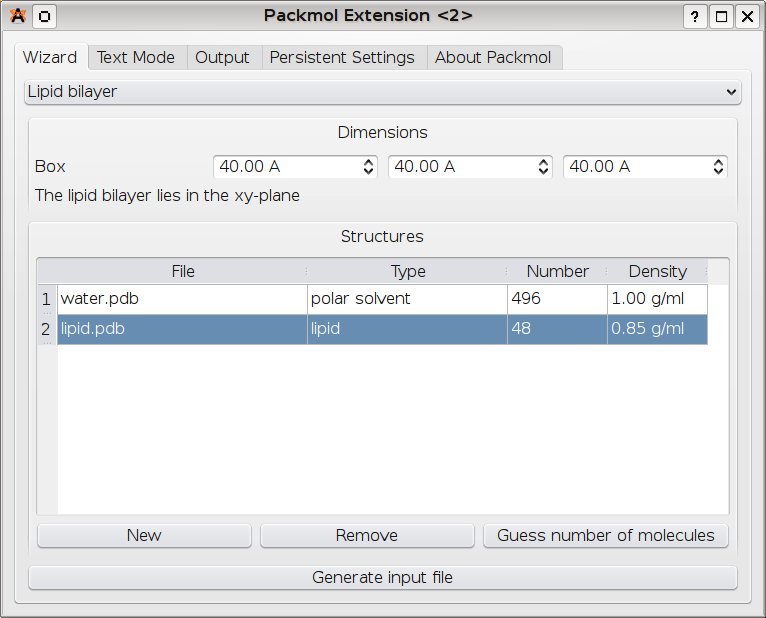
\includegraphics[width=0.45\textwidth]{images/packmol-extension}
  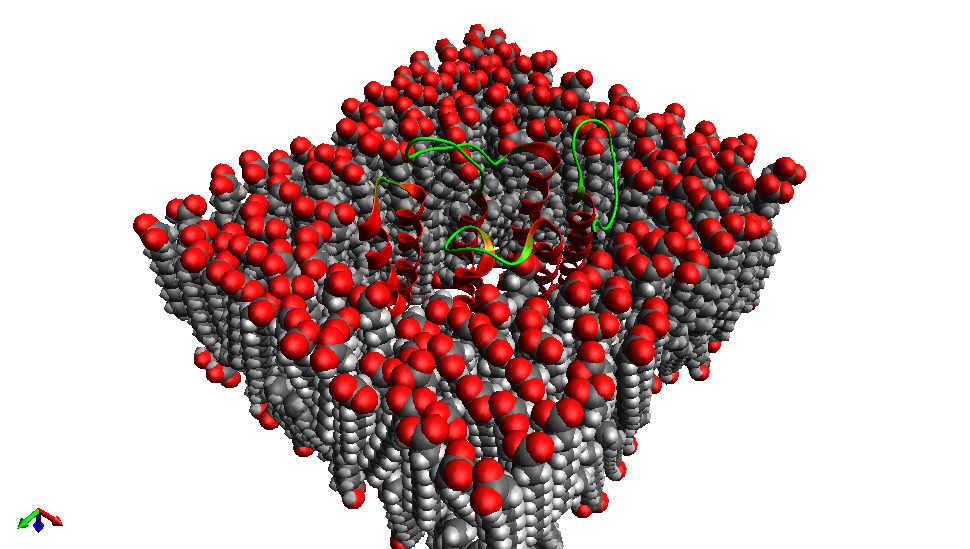
\includegraphics[width=0.45\textwidth]{images/packmol-lipid}
  \caption{The PackMol extension for Avogadro (left) and a lipid layer (right)
    as produced by the PackMol program.}
  \label{f:packmol}
\end{figure}

\subsection{XtalOpt}

\begin{figure}
  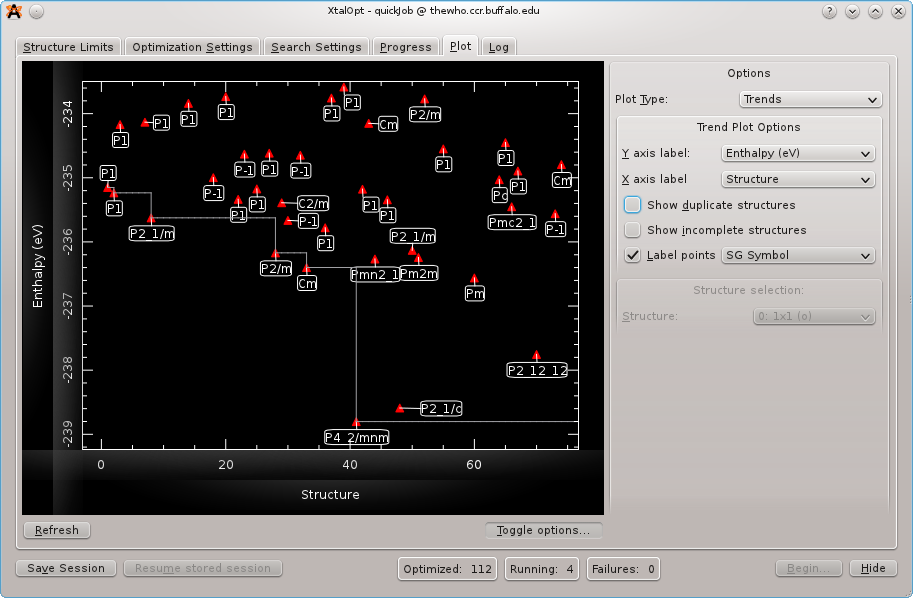
\includegraphics[width=0.95\textwidth]{images/xtalopt}
  \caption{The XtalOpt package showing a plot of stability vs. search progress
    for a $\mathrm{TiO_2}$ supercell.}
  \label{f:xtalopt}
\end{figure}

The XtalOpt~\cite{xo1, xo2} software package is implemented as a third-party C++
extension to Avogadro and makes heavy use of the libavogadro API. The extension
implements an evolutionary algorithm tailored for crystal structure prediction.
The XtalOpt development team chose Avogadro as a platform because of its
open source license, well-designed API, powerful visualization tools, and
intuitive user-interface. XtalOpt exists as a dialog window
(Figure~\ref{f:xtalopt}) and uses the main Avogadro window for visualizing
candidate structures as they evolve. The API is well suited for XtalOpt’s needs,
providing a simple mechanism to allow the user to view, edit, and export the
structures generated during the search. Taking advantage of the cross-platform
capabilities of Avogadro and its dependencies, XtalOpt is available for Linux,
Windows, and Mac.

\section{Conclusions}

\section{Availability and Requirements}

\textbf{Project Name:} Avogadro \\
\textbf{Project home page:} http://avogadro.openmolecules.net/ \\
\textbf{Operating system(s):} Cross-platform \\
\textbf{Programming language:} C++, bindings to Python \\
\textbf{Other requirements (if compiling):} CMake 2.4+ \\
\textbf{License:} GNU GPL v2 \\
\textbf{Any restrictions to use by non-academics:} None

\section{Acknowledgements and Funding}

We wish to thank the many contributors to the Avogadro project, including
developers, testers, translators, and users. We thank SourceForge for
providing resources for issue tracking and managing releases, and
Kitware for additional dashboard resources. MDH and GRH thank the
University of Pittsburgh for support. MDH also thanks Kitware and the
Engineering Research Development Center for support.

\section{Authors' contributions}
GRH and DEC are the founders of the Avogadro project. MDH is the
current lead developer and maintainer of Avogadro. DL and TV are
active developers. DL and EZ are founders of the XtalOpt project which
is discussed in this work. All authors read and approved the final manuscript.

\section{Competing interests}

The authors declare that they have no competing interests.

%%%%%%%%%%%%%%%%%%%%%%%%%%%%%%%%%%%%%%%%%%%%%%%%%%%%%%%%%%%%%
%%                  The Bibliography                       %%
%%                                                         %%
%%  Bmc_article.bst  will be used to                       %%
%%  create a .BBL file for submission, which includes      %%
%%  XML structured for BMC.                                %%
%%  After submission of the .TEX file,                     %%
%%  you will be prompted to submit your .BBL file.         %%
%%                                                         %%
%%                                                         %%
%%  Note that the displayed Bibliography will not          %%
%%  necessarily be rendered by Latex exactly as specified  %%
%%  in the online Instructions for Authors.                %%
%%                                                         %%
%%%%%%%%%%%%%%%%%%%%%%%%%%%%%%%%%%%%%%%%%%%%%%%%%%%%%%%%%%%%%

\newpage
{\ifthenelse{\boolean{publ}}{\footnotesize}{\small}
 \bibliographystyle{bmc_article}  % Style BST file
  \bibliography{AvogadroPaper} }     % Bibliography file (usually '*.bib' )

%%%%%%%%%%%

\ifthenelse{\boolean{publ}}{\end{multicols}}{}

\end{bmcformat}
\end{document}
